%
% This is a borrowed LaTeX template file for lecture notes for CS267,
% Applications of Parallel Computing, UCBerkeley EECS Department.
% Now being used for CMU's 10725 Fall 2012 Optimization course
% taught by Geoff Gordon and Ryan Tibshirani.  When preparing 
% LaTeX notes for this class, please use this template.
%
% To familiarize yourself with this template, the body contains
% some examples of its use.  Look them over.  Then you can
% run LaTeX on this file.  After you have LaTeXed this file then
% you can look over the result either by printing it out with
% dvips or using xdvi. "pdflatex template.tex" should also work.
%

\documentclass[twoside]{article}
\setlength{\oddsidemargin}{0.25 in}
\setlength{\evensidemargin}{-0.25 in}
\setlength{\topmargin}{-0.6 in}
\setlength{\textwidth}{6.5 in}
\setlength{\textheight}{8.5 in}
\setlength{\headsep}{0.75 in}
\setlength{\parindent}{0 in}
\setlength{\parskip}{0.1 in}

%
% ADD PACKAGES here:
%

\usepackage{amsmath,amsfonts,graphicx}

%
% The following commands set up the lecnum (lecture number)
% counter and make various numbering schemes work relative
% to the lecture number.
%
\newcounter{lecnum}
\renewcommand{\thepage}{\thelecnum-\arabic{page}}
\renewcommand{\thesection}{\thelecnum.\arabic{section}}
\renewcommand{\theequation}{\thelecnum.\arabic{equation}}
\renewcommand{\thefigure}{\thelecnum.\arabic{figure}}
\renewcommand{\thetable}{\thelecnum.\arabic{table}}

%
% The following macro is used to generate the header.
%
\newcommand{\lecture}[4]{
   \pagestyle{myheadings}
   \thispagestyle{plain}
   \newpage
   \setcounter{lecnum}{#1}
   \setcounter{page}{1}
   \noindent
   \begin{center}
   \framebox{
      \vbox{\vspace{2mm}
    \hbox to 6.28in { {\bf EE302 - Feedback Systems
	\hfill Spring 2019} }
       \vspace{4mm}
       \hbox to 6.28in { {\Large \hfill Lecture #1 \hfill} }
       \vspace{2mm}
       \hbox to 6.28in { {\it Lecturer: #2 \hfill } }
      \vspace{2mm}}
   }
   \end{center}
   \markboth{Lecture #1}{Lecture #1}

   \vspace*{4mm}
}
%
% Convention for citations is authors' initials followed by the year.
% For example, to cite a paper by Leighton and Maggs you would type
% \cite{LM89}, and to cite a paper by Strassen you would type \cite{S69}.
% (To avoid bibliography problems, for now we redefine the \cite command.)
% Also commands that create a suitable format for the reference list.
\renewcommand{\cite}[1]{[#1]}
\def\beginrefs{\begin{list}%
        {[\arabic{equation}]}{\usecounter{equation}
         \setlength{\leftmargin}{2.0truecm}\setlength{\labelsep}{0.4truecm}%
         \setlength{\labelwidth}{1.6truecm}}}
\def\endrefs{\end{list}}
\def\bibentry#1{\item[\hbox{[#1]}]}

%Use this command for a figure; it puts a figure in wherever you want it.
%usage: \fig{NUMBER}{SPACE-IN-INCHES}{CAPTION}
\newcommand{\fig}[3]{
			\vspace{#2}
			\begin{center}
			Figure \thelecnum.#1:~#3
			\end{center}
	}
% Use these for theorems, lemmas, proofs, etc.
\newtheorem{theorem}{Theorem}[lecnum]
\newtheorem{lemma}[theorem]{Lemma}
\newtheorem{proposition}[theorem]{Proposition}
\newtheorem{claim}[theorem]{Claim}
\newtheorem{corollary}[theorem]{Corollary}
\newtheorem{definition}[theorem]{Definition}
\newenvironment{proof}{{\bf Proof:}}{\hfill\rule{2mm}{2mm}}

% **** IF YOU WANT TO DEFINE ADDITIONAL MACROS FOR YOURSELF, PUT THEM HERE:

\begin{document}

% Lecture Details
\lecture{1}{Asst. Prof. M. Mert Ankarali}

\par 

\section*{Dynamical Systems}

A dynamical system is a collection of ``elements'' for which 
there is a time-dependent cause and effect relationships between
``variables''. The behavior of a dynamical system changes with time, 
usually in response to external inputs. 

The elements can range from atoms and molecules to
oceans and planets. Similarly, time scales can range from
pico seconds to years and even decades.

\subsection*{Modeling of Dynamical Systems}

\textbf{Goal:} Obtaining a mathematical description of the 
dynamic relationship between the variables of the given 
dynamical system/behavior. \textbf{\textit{Always}}, 
the mathematical description is a simplification of the 
real phenomena. Always remember:

\par

``All models are wrong but some are useful'' George E. Box, 1978.

\par

\vspace{6pt}

\textbf{Representations of (Continious-Time) Dynamical Systems}

\begin{enumerate}
  \item Differential equations

\begin{align*}
a_n  y^{(n)} + ... + a_1 y' + a_0 y = b_{n}  u^{(n)} + ... + b_1 u' + b_0 u 
\end{align*}

Differential equations can model both linear and non-linear systems,
time-invariant and time-varying ones. 

  \item Impulse response representation

\begin{align*}
  y(t) &= h(t) \ast u(t) = \int\limits_{-\infty}^{\infty} h(t-\tau) u(\tau) d\tau 
\end{align*}

Impulse-response representation can be used to model the dynamic
relation between input, $u(t)$, and output $y(t)$ signals. 
This reprsentation is limited to Linear-Time-Invariant (LTI) systems. 

\par

Time varying impulse response representation can be used to model 
Linear-Time-Varying (LTV) systems.

\item Transfer function representation 

\begin{align*}
  Y(s) &= G(s) U(s) , \ \mathrm{where}  , \\
  Y(s) &= \mathcal{L}\lbrace y(t) \rbrace \ , \& \   
  U(s) = \mathcal{L}\lbrace u(t) \rbrace
\end{align*}

Transfer functions are limited to LTI systems. 

\item State-space representation

\begin{align*}
  \mathrm{Let} \ x(t) &\in \mathbb{R}^n \ , \ y(t) \in \mathbb{R} \ ,\  u(t) \in
  \mathbb{R} , \\
  \dot{x}(t) &= A x(t) + B u(t) , \\
  y(t) &= C x(t) + D u(t) , \\
  \mathrm{where} \ A &\in \mathbb{R}^{n \times n} \ , \ 
    B \in \mathbb{R}^{n \times 1} \ ,\  C \in \mathbb{R}^{1 \times n} \ , \ D \in \mathbb{R}
\end{align*}

Similar to differential equations, we can model both linear and non-linear systems,
and time-invariant and time-varying systems using state-space representations.

\end{enumerate}

\subsection*{Feedback Systems}

The \textit{feedback} terms constitute to the case, where 
dynamical systems are connected in a way that the output of each 
the system influences its own driving input (directly or indirectly)
and dynamic relations between different sub-systems are 
tightly coupled. 

Simple causal reasoning about a feedback system is difficult (if not possible). For example, if we observe the feedback system illustrated in Fig. \ref{fig:closed_open}(B), we see that the first system influences the second, and the second system influences the first, leading to a circular argument. We can conclude that formal methods are necessary to understand the behavior of feedback systems. 

Fig.~\ref{fig:closed_open} illustrates the idea of feedforward vs. feedback in block diagram topology. Open-loop and closed-loop terms are also commonly used to refer to feedforward and feedback structures, respectively.  When systems connect each other in a cyclic topology, we refer to the topolgy as a closed-loop system. If one cuts an interconnection such that the cyclic structure is broken, the system becomes an open-loop system.

\begin{figure}[h]
	\centering
	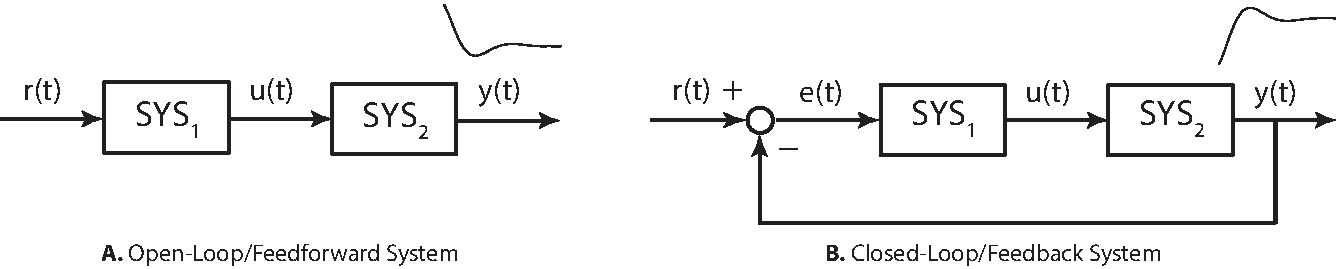
\includegraphics[width=\textwidth]{closed_openloop}
	\caption{Open- and closed-loop systems}
	\label{fig:closed_open}
\end{figure}

Feedback based control may not be mandatory for some control applications, yet a feedforward based control policy can be more
advantageous than a feedback-based control policy in some cases. 
The core benefit of feedback in a control system is that feedback
reduces uncertainties in systems and improves the robustness. 
Since uncertainties are unavoidable in real life, feedback
control systems are ubiquitous in both synthetic and biological
control systems. 

\section*{Dynamic Modeling of Some Physical Systems}

\subsection*{Electrical Circuits}

\textbf{Ex 1: Series RLC Circuit}

Given than input is $u(t) = V_s(t)$ and output os $y(t) = V_C(t)$, find an ODE 
description of the given dynamical circuit. 

  \begin{minipage}[h]{0.5\linewidth}
    \begin{center}
      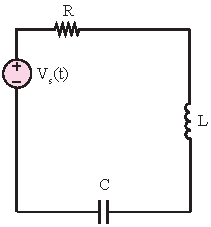
\includegraphics[width=0.75\textwidth]{RLC}
    \end{center}
  \end{minipage}
  \begin{minipage}[h]{0.5\linewidth}
    \begin{center}
    {\large
  \begin{align*}
  	V_L + V_R + V_C &= V_s(t)
	\\
	L \frac{d I}{dt} + R I + V_C &= V_s(t)
	\\
	L \frac{d }{dt} \left( C \frac{d V_C}{dt} \right) + R  \left( C \frac{d V_C}{dt} \right) + V_C &= V_s(t)
	\\
	LC \ \ddot{V}_C + RC \ \dot{V_C} + V_C &= V_s(t)
	\\
	\ddot{y} + \frac{R}{L} \dot{y} + \frac{1}{LC} y &= \frac{1}{LC} u
  \end{align*}
  }
    \end{center}
  \end{minipage}

Find the transfer function representation of the system for the given input--output pair.
%
\begin{align*}
	\mathcal{L} \left\lbrace \ddot{y} + \frac{R}{L} \dot{y} + \frac{1}{LC} y  \right\rbrace 
	&= \mathcal{L} \left\lbrace \frac{1}{LC} u  \right\rbrace
	\\
	s^2 Y(s) + s \frac{R}{L} Y(s) + \frac{1}{LC} Y(s) &=  \frac{1}{LC} U(s) \\
	G(s) = \frac{Y(s)}{U(s)} &= \frac{\frac{1}{LC} }{s^2 + \frac{R}{L} s + \frac{1}{LC} }
\end{align*}

Find a state-space representation of the system.

\par

Let $x = \left[ \begin{array}{c} x_1 \\ x_2 \end{array} \right] = \left[ \begin{array}{c} y \\ \dot{y} \end{array} \right]$, then 
%
\begin{align*}
	\dot{x_1} &= x_2 \\
	\dot{x_2} &= -\frac{1}{LC} x_1 - \frac{R}{L} x_2 + \frac{1}{LC} u
\end{align*}
%
If we put the equations in state-space form, we obtain
%
\begin{align*}
 \dot{x} &= \left[  \begin{array}{cc} 0 & 1 \\ -\frac{1}{LC} &  -\frac{R}{L}  \end{array} \right] x 
 +  \left[  \begin{array}{c} 0 \\ \frac{1}{LC} \end{array} \right] u
 \\
 y &= \left[  \begin{array}{cc} 1 & 0 \end{array} \right] x 
\end{align*}
%
where
%
\begin{align*}
 A = \left[  \begin{array}{cc} 0 & 1 \\ -\frac{1}{LC} &  -\frac{R}{L}  \end{array} \right] \quad , \
 B = \left[  \begin{array}{c} 0 \\ \frac{1}{LC} \end{array} \right]  \quad , \
 C = \left[  \begin{array}{cc} 1 & 0 \end{array} \right] \quad , \
 D = 0
\end{align*}

Now let, $z = \left[ \begin{array}{c} z_1 \\ z_2 \end{array} \right] =
\left[ \begin{array}{c} V_C \\ I \end{array} \right]$, then 
%
\begin{align*}
	\dot{z_1} &= \frac{1}{C} z_2 \\
	\dot{z_2} &= -\frac{1}{L} z_1 - \frac{R}{L} z_2 + \frac{1}{L} u
\end{align*}
%
If we put the equations in state-space form, we obtain
%
\begin{align*}
 \dot{z} &= \left[  \begin{array}{cc} 0 & \frac{1}{C} \\ -\frac{1}{L} &  -\frac{R}{L}  \end{array} \right] z 
 +  \left[  \begin{array}{c} 0 \\ \frac{1}{L} \end{array} \right] u
 \\
 y &= \left[  \begin{array}{cc} 1 & 0 \end{array} \right] z
\end{align*}
%
It can be seen that state-space representation of a dynamical system
is not unique. Indeed there exist ifinitelly many state-space
representations of the same system.
%


% **** This ENDS THE EXAMPLES. DON'T DELETE THE FOLLOWING LINE:
\end{document}